\chapter{Life Is Sacred}

This chapter follows the last movement of the Brockwood Park dialogue of 20 May 1976, in which J. Krishnamurti and his interlocutors ask whether the ending of image, thought, and sorrow opens onto compassion, silence, and the sacred. There are no blackboard equations in the source material. The mathematical language used here is therefore schematic: a way of preserving distinctions, dependencies, and turns in the inquiry without turning the dialogue into a doctrine.

\section{The Blank Wall After Negation}

The lecture begins after a clearing has already taken place. The outsider has listened, has seen through systems, gurus, and prepared meditations, and has understood that the meditator is not separate from meditation. He has been left without future, without past, without image. The result is not triumph. It is a blank wall.

This is the right starting point. If all the old maps of happiness have been set aside, the first question is not whether the argument is elegant. The first question is whether life can be lived from this emptiness. One participant asks, in effect, how one is to get out of bed in the morning. That question is dismissed as simple only in a limited sense: life demands that we act. We cannot merely stay in bed because our theories have collapsed.

But that does not settle the deeper matter. Action may still be routine, conformity, or reaction. The outsider is asking for something more exact: has sorrow ended, is there love, is there compassion, and has death been understood?

We can record the initial state as a schematic clearing:
\begin{equation}
\text{systems, gurus, methods, images}
\quad \longrightarrow \quad
\text{discarded}
\quad \longrightarrow \quad
\text{blank wall}.
\end{equation}
This is not a formula for liberation. It is the first condition of the inquiry. The negation of false maps leaves a space, and the dialogue asks what, if anything, that space contains.

\section{What Dies When the Self Is an Image?}

The first explicit problem is death. The morning dialogue had reached the point that when the observer is seen as the observed, something like death is involved. Now the question is pressed more sharply: if the self is nothing but an image, what is it that dies?

There is biological death, the death of the organism. The speakers acknowledge it, but they are not primarily discussing it. They are asking whether the ending of the psychological self-image is death in any deep sense. If the image is fictitious, then the mere ending of the image may seem too trivial. It may be like turning off a television: something stops, but nothing real has died.

The first distinction is therefore:
\begin{equation}
\text{death}_{\mathrm{bio}}
\neq
\text{death}_{\mathrm{psych}}.
\end{equation}
Biological death is the ending of the organism. Psychological death is being explored as the ending of image, thought, memory, time, and accumulation.

But the dialogue immediately refuses a shallow version:
\begin{equation}
\text{death}_{\mathrm{psych}}
\neq
\text{mere ending of image}.
\end{equation}
That inequality is the first real hinge of the chapter. The death of image is acknowledged, but the dialogue insists that death must have a much wider significance.

\subsection{Question \& Answer}

\paragraph{Question.}
If the self is an image, and the image ends, what has really died?

\paragraph{Answer.}
At first, only the image has ended. That may be necessary, but it is not yet the full meaning of death. The image has been taken as real, and therefore its ending can feel frightening; nevertheless, if it is only the image that ends, the inquiry remains shallow. The dialogue therefore asks for the ending of something deeper than the image.

\paragraph{Working distinction.}
We can place the first three layers side by side:
\begin{align}
\text{organism ends} &\quad \Rightarrow \quad \text{biological death}, \\
\text{image ends} &\quad \Rightarrow \quad \text{a shallow psychological ending}, \\
\text{known ends} &\quad \Rightarrow \quad \text{the deeper question of death}.
\end{align}
The third line is not yet fully explained. It is where the dialogue is going.

\section{Image, Thought, Time, and the Known}

The next step is to ask what lies behind the image. The answer given in the dialogue is thought. Thought is the maker of image. If the self-image dies but the maker of images continues, the root has not ended.

The sequence can be written as a conceptual ladder:
\begin{equation}
\text{image}
\longrightarrow
\text{image-maker/thought}
\longrightarrow
\text{memory and concepts}
\longrightarrow
\text{psychological time}
\longrightarrow
\text{the known}.
\end{equation}
The arrow here means ``leads the inquiry toward,'' not mechanical causation. Krishnamurti is not constructing a formal psychology. He is showing why a merely verbal ending is insufficient.

The dialogue then asks why death should matter to the whole of life. The answer is that death, in the psychological sense being examined, means the ending of everything known: reality as thought has built it, concepts, images, memories, and the movement of time as past continuing through the present into the future. Clock time remains. The psychological future, made by the past carrying itself forward, is the issue.

A compact way to mark this distinction is:
\begin{align}
\text{clock time} &\neq \text{psychological time}, \\
\text{psychological time} &\sim \text{past meeting the present and carrying on}.
\end{align}
The word ``sim'' is deliberate. We are not defining time in general. We are marking the way the dialogue uses the phrase.

\begin{proposition}
In the dialogue, death becomes philosophically significant only when it is not restricted to biological ending or image-ending, but is understood as the ending of the psychological known.
\end{proposition}

\begin{proof}
The dialogue first distinguishes biological death from the death under discussion. It then tests the ending of image and rejects it as too shallow. It next identifies thought as the image-maker and includes memory, concept, and psychological time in the field that must end. Therefore the significant sense of death is not the mere disappearance of an image but the ending of the accumulated known.
\end{proof}

\section{The Stream of Image-Making}

At this point the inquiry changes scale. If the organism dies while image-making remains, does that image-making simply vanish with one brain? The dialogue suggests not. The image is not fundamentally private. My image and your image may have different frills and colors, but essentially they belong to the same stream.

This is one of the most important turns in the lecture. The problem is no longer only ``my'' image. There is a constant flow of image-making. It manifests through people. It is not merely a private possession.

We can draw the point as a transcript-derived schematic, not as a board diagram.

\begin{figure}
\centering
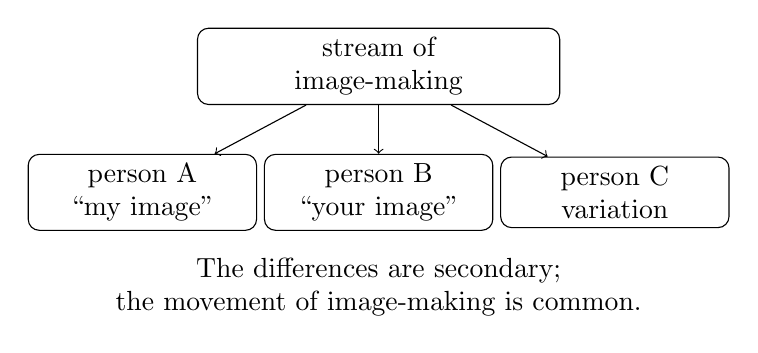
\begin{tikzpicture}[x=1cm,y=1cm]
\node[draw, rounded corners, align=center, minimum width=4.6cm, minimum height=0.85cm] (stream) at (0,0) {stream of\\ image-making};
\node[draw, rounded corners, align=center, minimum width=2.9cm, minimum height=0.75cm] (p1) at (-3,-1.6) {person A\\ ``my image''};
\node[draw, rounded corners, align=center, minimum width=2.9cm, minimum height=0.75cm] (p2) at (0,-1.6) {person B\\ ``your image''};
\node[draw, rounded corners, align=center, minimum width=2.9cm, minimum height=0.75cm] (p3) at (3,-1.6) {person C\\ variation};
\draw[->] (stream) -- (p1);
\draw[->] (stream) -- (p2);
\draw[->] (stream) -- (p3);
\node[align=center] at (0,-2.8) {The differences are secondary;\\ the movement of image-making is common.};
\end{tikzpicture}
\caption{A schematic reconstruction of the dialogue's river image: image-making is treated as a common stream manifesting through persons.}
\end{figure}

The immediate payoff is that death cannot be understood if we remain confined to the private image. If the individual image is a small eddy in a larger movement, then the ending of one image is still not the whole of death. The inquiry must move into the stream itself.

\section{Universal Sorrow Beneath the Surface}

The stream metaphor deepens. Image-making is now described as a surface movement, like waves on a river. Beneath it is sorrow. This sorrow is not merely pain, not merely loss, not merely the grief of losing a parent or child, and not merely self-pity. It is much deeper than thought and ordinary feeling.

The distinction can be marked in schematic notation:
\begin{equation}
\text{sorrow}_{\mathrm{thought}}
\neq
\text{universal sorrow}.
\end{equation}
Thought-made sorrow includes self-pity and the personal drama of the image. Universal sorrow is the deeper sorrow of mankind: ignorance, destruction, repeated wars, poverty, and the long continuity of human beings mistreating one another.

The dialogue asks whether the stream of sorrow is different from the stream of image-making. The answer is subtle. It is not a second stream. It is the same stream at a deeper level. Image-making is the surface wave; sorrow is the depth out of which the surface disturbance comes.

\begin{figure}
\centering
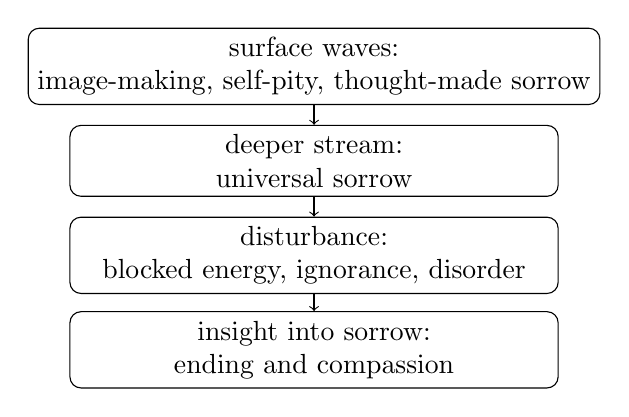
\begin{tikzpicture}[x=1cm,y=1cm]
\node[draw, rounded corners, align=center, minimum width=6.2cm, minimum height=0.75cm] (waves) at (0,1.2) {surface waves:\\ image-making, self-pity, thought-made sorrow};
\node[draw, rounded corners, align=center, minimum width=6.2cm, minimum height=0.75cm] (stream) at (0,0) {deeper stream:\\ universal sorrow};
\node[draw, rounded corners, align=center, minimum width=6.2cm, minimum height=0.75cm] (disturb) at (0,-1.2) {disturbance:\\ blocked energy, ignorance, disorder};
\node[draw, rounded corners, align=center, minimum width=6.2cm, minimum height=0.75cm] (insight) at (0,-2.4) {insight into sorrow:\\ ending and compassion};
\draw[->] (waves) -- (stream);
\draw[->] (stream) -- (disturb);
\draw[->] (disturb) -- (insight);
\end{tikzpicture}
\caption{A pocket-size schematic of the stream metaphor. It is not a physical model; it records the dialogue's order of distinctions.}
\end{figure}

\subsection{Question \& Answer}

\paragraph{Question.}
Is universal sorrow a different stream from image-making?

\paragraph{Answer.}
No. The dialogue treats it as part of the same stream, but much deeper. Image-making is surface wave activity. The sorrow of mankind is the deeper current. Disturbances in that depth show themselves at the surface as image, self-pity, fear, anxiety, and confusion.

\paragraph{Worked example.}
Suppose we use a simple two-level notation:
\begin{align}
W &= \text{surface waves: image-making and self-pity}, \\
D &= \text{deeper current: universal sorrow}.
\end{align}
A shallow account studies only $W$. The dialogue insists that a serious inquiry must not stop there:
\begin{equation}
W \subset \text{movement of the stream}, 
\qquad
D \subset \text{movement of the stream},
\qquad
D \text{ is deeper than } W.
\end{equation}
The notation is only a reading aid. Its purpose is to prevent the final chapter from collapsing universal sorrow into private unhappiness.

\section{Compassion and the Ending of Sorrow}

The lecture now asks what compassion is. The word is linked with love, but the dialogue uses it with great care. Compassion is not pity. It is not sentimental sorrow for another person. It is not the outcome of going through every horror of mankind. That formulation is explicitly resisted.

The key correction is this: compassion is born of sorrow only in the sense that when the deeper sorrow ends, compassion is. The enlightened one sees sorrow and destruction, but is not himself caught in sorrow. He senses a tremendous energy; the dialogue calls that compassion.

A cautious schematic is:
\begin{equation}
\text{ending of deeper sorrow}
\longrightarrow
\text{compassion}
\longrightarrow
\text{energy}.
\end{equation}
Even this arrow must be handled carefully. It is not a recipe. It is the order in which the dialogue clarifies the relation.

\subsection{Question \& Answer}

\paragraph{Question.}
Must one first pass through sorrow in order to have compassion?

\paragraph{Answer.}
No. The dialogue rejects that implication. One need not pass through all the horrors of mankind as a personal sequence. The corrected point is that compassion is not available while the mind remains in thought-made sorrow, self-pity, and image. When the deeper sorrow ends, there is compassion.

\paragraph{Update rule for the draft.}
Whenever the chapter is tempted to write
\begin{equation}
\text{sorrow} \longrightarrow \text{compassion},
\end{equation}
it should replace that with the more precise form:
\begin{equation}
\text{ending of sorrow}
\longrightarrow
\text{compassion}.
\end{equation}
And even this must be qualified: the sorrow in question is not merely personal sorrow or self-pity, but the deeper sorrow of mankind.

The dialogue then introduces a further image: energy caught in whirlpools, or a vast reservoir of sorrow moving in a disorderly way. This must not be over-modeled. It means that deep sorrow is not a calm object to be inspected from outside; it is a disorder in the movement of life that perpetuates ignorance. If it were not for that disorder, perhaps man's natural capacity to learn would resolve the problems.

\section{Silence, Emptiness, and Energy}

The lecture next returns to death, but now death is no longer merely the ending of image or thought. It is the opening into something beyond death. The speakers ask whether this is eternal, then correct the word toward ``beyond time.'' They speak of a movement with no beginning and no ending, a movement not in time.

This is not the movement of sequence:
\begin{equation}
\text{movement in time}
\neq
\text{movement beyond time}.
\end{equation}
The first belongs to duration, transition, and continuity. The second is described as constant renewal, freshness, flowering, without becoming old.

The practical condition for entering this is stated with exceptional clarity: the mind must be completely silent. But silence is not produced by control. It is not wished for, premeditated, predetermined, or brought about through will. Otherwise the mind would merely be projecting another image into the unknown.

The sequence becomes:
\begin{equation}
\text{absolute silence}
\longrightarrow
\text{nothing}
\longrightarrow
\text{emptiness}
\longrightarrow
\text{tremendous energy}.
\end{equation}
Then comes an important correction. One speaker asks whether this is the source of compassion. The answer does not rest with the language of source. The more exact statement is:
\begin{equation}
\text{energy} = \text{compassion}.
\end{equation}
This equality is not physics. It is a strong verbal identity within the dialogue. The word energy does not refer to a measurable quantity. It names the living intensity present when the mind is empty of projection, control, image, and time.

\section{The Sacred and the Question of Sharing}

Having reached compassion, the dialogue asks whether there is something beyond it. The answer is the sacred. But the sacred is approached negatively, and that negative approach is essential. Everything thought has created is not sacred. An image of worship, a holy symbol made by hand or mind, remains an image. Thought is fragmented, limited, finite, and memory-bound; therefore what thought creates cannot be the sacred.

We can write the distinction sharply:
\begin{align}
\text{thought-created sacred} &= \varnothing, \\
\text{sacred} &\notin \text{products of thought}.
\end{align}
The first line is not meant literally as set theory. It is a compact warning: do not mistake thought's object for the sacred.

The dialogue then asks about relationship. What is the relation between reality, which is the product of thought, and that which is sacred? Reality in this restricted sense has no relation to the sacred. Relationship comes, if at all, through insight, intelligence, and compassion. Intelligence here is not cleverness. It is insight into image, into thought, into sorrow, and then into compassion. It is not yours or mine.

The movement can be summarized:
\begin{equation}
\text{insight}
\longrightarrow
\text{intelligence}
\longrightarrow
\text{compassion}
\longrightarrow
\text{sacred}.
\end{equation}
But the last arrow is delicate. The sacred is not an object reached by a procedure. Krishnamurti says that a living thing cannot be examined as a dead thing. The notes should therefore keep the arrow as a reading aid, not a technique.

The closing question is whether the viewer has merely heard a clever discussion or has shared in the meditation of the dialogue. The speakers ask whether the bowl has been filled with the sacred or whether only ashes remain. They ask whether the dialogue has shared the perfume of the thing, not merely its verbal remains.

The final identification is simple and severe:
\begin{equation}
\text{life} = \text{sacred}.
\end{equation}
Again, this is not a doctrine to be accepted as a theory. The dialogue immediately warns that accepting it as theory is no better than accepting any other theory. If life is sacred, then life must not be misused or wasted. Each life is part of the whole.

\subsection{Question \& Answer}

\paragraph{Question.}
Has the dialogue shared the sacred, or only words about the sacred?

\paragraph{Answer.}
That is the burning question at the end. If the dialogue is only clever argument, nothing essential has been shared. But if the dialogue itself has been meditation, then sharing is no longer one person giving something to another. The final movement points beyond speaker, viewer, and possession: there is only that.

\section{Summary}

This lecture moves by refusing premature closure. The ending of systems leaves a blank wall. The ending of image is not yet death. The ending of thought is still not deep enough. The stream of image-making leads into the deeper stream of sorrow. The ending of deeper sorrow is compassion, and compassion is energy. Silence, not produced by will, opens into emptiness; emptiness is not barrenness but tremendous energy.

The sacred is not made by thought, not captured by an image, and not examined as an object. The dialogue ends by asking whether all this has been shared as living meditation or merely discussed. Its final claim is not a consoling idea about happiness. It is the stark identification that life is sacred, and that to treat life as a theory is already to miss it.